\documentclass[twocolumn]{article}

\usepackage{amsmath}
\usepackage{subfigure}
\usepackage{fullpage}
\usepackage{graphicx}

\author{Ana Laura Sarracino Ortiz}
\date{Jul 4$^{\text{th}}$ 2016}

\title{\sc La ecuaci\'on de Schr\"odinger}

\begin{document}
\maketitle{}

\section{Erwin Schr\"odinger}
Erwin Rudolf Josef Alexander Schr\"odinger(\ref{fig:erwin}), fue un f\'isico austr\'iaco, naturalizado irland\'es, que realiz\'o importantes contribuciones en los campos de la mec\'anica cu\'antica y la termodin\'amica. Recibi\'o el Premio Nobel de F\'isica en 1933 por haber desarrollado la ecuaci\'on de Schr\"odinger. Tras mantener una larga correspondencia con Albert Einstein propuso el experimento mental del gato de Schr\"odinger que mostraba las paradojas e interrogantes a los que abocaba la f\'isica cu\'antica.

\begin{figure}[h!b]
	\centering
	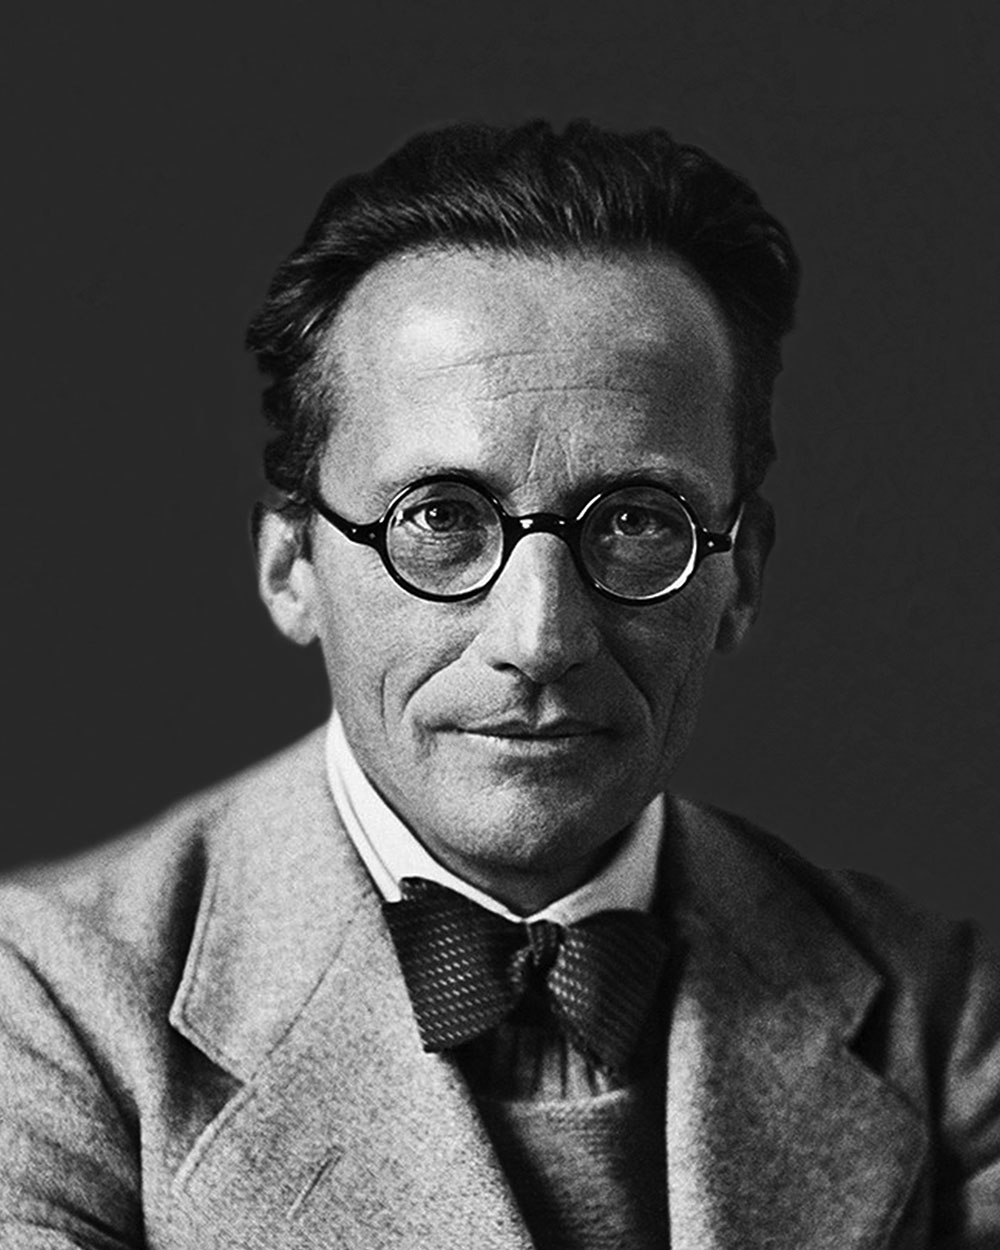
\includegraphics[width=0.3\textwidth]{Erwin}
	\caption{Erwin Rudolf Josef Alexander Schrodinger}
	\label{fig:erwin}
\end{figure}


\section{Introducci\'on}
La ecuaci\'on de Schr\"odinger desempe\~na el papel de las leyes de Newton y la
conservaci\'on de la energ\'ia de la mec\'anica cl\'asica, es decir, predice
el comportamiento futuro de un sistema din\'amico-. Se trata de una ecuaci\'on
de onda en t\'erminos de la funci\'on de onda, que predice anal\'iticamente y
con precisi\'on, la probabilidad de eventos o resultados. El resultado
detallado no est\'a estrictamente determinado, pero dado un gran n\'umero de
eventos, la ecuaci\'on de Schr\"odinger predice la distribuci\'on de los
resultados. La ecuaci\'on de Schr\"odinger, en su forma m\'as general(1), indica la variaci\'on que sufre un
estado f\'isico, a lo largo del tiempo, cuando el sistema que describe se encuentra
sometido a un hamiltoniano de la forma $\hat{H}$ . En estas condiciones, la ecuaci\'on de Schr\"odinger se
escribe en la forma(2):

\section{Equations}

    \begin{equation}
	i\hbar\frac{\partial{\psi}}{\partial{t}}(r,t)=\hat{H}{\psi}(r,t)
    \end{equation}	

    \begin{equation}
	\hat{H} \Psi= E \Psi
    \end{equation}

\end{document}

